\documentclass[conference]{IEEEtran}
\IEEEoverridecommandlockouts
\usepackage{cite}
\usepackage{amsmath,amssymb,amsfonts}
\usepackage{graphicx}
\usepackage{textcomp}
\usepackage{xcolor}
\usepackage{booktabs}
\usepackage{multirow}
\usepackage{url}
\usepackage[hidelinks]{hyperref}

\def\BibTeX{{\rm B\kern-.05em{\sc i\kern-.025em b}\kern-.08em
    T\kern-.1667em\lower.7ex\hbox{E}\kern-.125emX}}

\begin{document}

\title{
\includegraphics[height=1.9cm]{figs/logo_faculty_eng.png}\hspace{1.3cm}
\includegraphics[height=1.9cm]{figs/logo_cairo_univ.png}\\[10pt]
Explainable Machine Learning for Polycystic Ovary Syndrome Screening: A Comparative Evaluation of Model Performance, Feature Reduction, and Probability Calibration}

\author{
\IEEEauthorblockN{Habiba Abdelmeneem Ramadan Abdelmeneem}
\IEEEauthorblockA{
Systems and Biomedical Engineering Department \\
Faculty of Engineering, Cairo University \\
Giza, Egypt \\
}
}

\maketitle

\begin{abstract}
Polycystic ovary syndrome (PCOS) is one of the most common endocrine disorders among women of reproductive age, yet its diagnosis remains subjective due to overlapping symptoms and reliance on a combination of clinical, hormonal, and ultrasound criteria. This paper presents a machine learning pipeline for PCOS prediction that goes beyond raw predictive accuracy to examine model interpretability, feature efficiency, and probability reliability. Three classifiers -- Logistic Regression, Random Forest, and XGBoost -- were trained and evaluated on a publicly available clinical dataset of 541 patients. All three models achieved comparable discriminative performance (ROC-AUC 0.949--0.956), and a paired statistical test confirmed no significant difference between the top two models ($p = 0.322$). Using SHAP (SHapley Additive exPlanations) values, we identified a reduced set of 10 clinically interpretable features that retained statistically equivalent performance to the full 44-feature model ($p = 0.893$), with consistent feature rankings across all three model architectures. We further optimized the classification threshold to prioritize diagnostic recall (improving sensitivity from 77.8\% to 91.7\% at the cost of moderate precision), and performed calibration analysis revealing that the best-performing model (XGBoost) was the least reliable in terms of predicted-probability trustworthiness, while Logistic Regression -- despite lower raw accuracy -- was best calibrated. These findings suggest that model selection for clinical deployment should depend on intended use case, and that a compact, 10-feature model may offer a practical, lower-cost screening alternative in resource-limited settings. A working interactive prototype implementing the reduced model was deployed as a web application to demonstrate feasibility.
\end{abstract}

\begin{IEEEkeywords}
polycystic ovary syndrome, machine learning, explainable AI, SHAP, feature selection, model calibration, random forest, XGBoost, clinical decision support
\end{IEEEkeywords}

\section{Introduction}

Polycystic ovary syndrome (PCOS) is a hormonal disorder affecting approximately 8--13\% of women of reproductive age worldwide \cite{ghaderzadeh2025}. It is characterized by a combination of hyperandrogenism, ovulatory dysfunction, and polycystic ovarian morphology on ultrasound \cite{rotterdam2004}. Despite its prevalence, PCOS remains substantially under-diagnosed and frequently delayed, in part because no single test can confirm it: clinical diagnosis relies on the Rotterdam criteria, which require any two of three qualitative findings, and different clinicians may weigh overlapping and non-specific symptoms -- irregular cycles, acne, weight gain, excess hair growth -- inconsistently \cite{rotterdam2004}.

This diagnostic ambiguity has motivated a growing body of work applying machine learning (ML) to PCOS detection. Recent systematic reviews report that supervised ML classifiers and imaging-based deep learning models consistently outperform traditional rule-based diagnostic approaches in retrospective evaluations, reducing the subjectivity inherent in manual assessment \cite{ghaderzadeh2025, barrera2023}. However, the same reviews highlight persistent gaps: only a minority of published PCOS-ML studies apply explainable AI (XAI) techniques, most report a single train/test split without statistical validation of model comparisons, and probability calibration -- whether a model's predicted risk score can be trusted at face value -- is rarely examined at all \cite{ghaderzadeh2025}. Several prior studies have proposed web-deployable PCOS prediction tools using classical classifiers with basic feature selection \cite{webbased2024, mohiuddin2025}, demonstrating clinical feasibility but generally without rigorous statistical comparison between models or between full and reduced feature sets.

This paper addresses these specific gaps. Rather than proposing a single new classifier, we ask three questions that are directly relevant to real-world, resource-constrained deployment of PCOS screening tools:

\begin{enumerate}
    \item Do different model architectures (linear vs. tree-based) actually differ significantly in predictive performance, or only numerically?
    \item Can the feature set required for diagnosis be meaningfully reduced without a statistically significant loss in performance, and is feature importance consistent across model types?
    \item Is the model with the highest raw accuracy also the model whose predicted probabilities can be trusted?
\end{enumerate}

We answer these questions using paired statistical significance testing, cross-model SHAP-based feature attribution, and calibration curve analysis -- and we translate the resulting 10-feature model into a working interactive screening prototype to demonstrate practical deployability.

\section{Related Work}

Barrera et al. \cite{barrera2023} conducted a systematic review of ML and AI applications in PCOS diagnosis and classification, finding that most published models achieve high reported accuracy but suffer from small, single-source datasets and limited external validation. Ghaderzadeh et al. \cite{ghaderzadeh2025} extended this analysis specifically to explainability, reporting that only approximately 25\% of reviewed PCOS-AI studies applied any XAI method (SHAP, LIME, or Grad-CAM), and explicitly identified standardized reporting and systematic use of XAI as priorities for future work.

Closer to the present study, Mohi Uddin \cite{mohiuddin2025} compared traditional and ensemble ML models for PCOS detection with feature selection, aiming to bridge ML performance with clinical applicability using established markers such as BMI, AMH, and cycle regularity. A separate study proposed a web-based interface integrating multiple classical classifiers (Logistic Regression, Naive Bayes, SVM, KNN) with mutual-information-based feature selection for early PCOS prediction \cite{webbased2024}. These works demonstrate that both model comparison and deployable interfaces are established directions in this space; the present work differentiates itself by combining statistical hypothesis testing of model differences, cross-architecture SHAP agreement analysis, explicit precision--recall threshold optimization, and calibration analysis within a single, internally consistent study -- and by reporting negative results (e.g., hyperparameter tuning yielding no improvement) transparently rather than only reporting favorable outcomes.

\section{Dataset and Methods}

\subsection{Dataset}

The primary dataset used in this study is a publicly available clinical PCOS dataset comprising 541 patients (364 PCOS-positive, 177 PCOS-negative) collected across multiple hospitals, with 44 clinical, hormonal, and ultrasound-derived features per patient, including follicle counts (left and right ovary), Anti-M\"{u}llerian Hormone (AMH) level, luteinizing hormone (LH), body mass index (BMI), menstrual cycle length and regularity, and self-reported symptoms such as weight gain, skin darkening, hirsutism, and acne \cite{kottarathil}.

\subsection{Preprocessing}

Column names were standardized, non-numeric artifacts were coerced to numeric type, and non-predictive identifier columns were removed. Missing values were imputed using median imputation. The dataset was split into training (80\%) and held-out test (20\%) partitions using stratified sampling to preserve class balance. Features used for Logistic Regression were standardized (zero mean, unit variance); tree-based models used unscaled features.

\subsection{Models}

Three classifiers were trained: Logistic Regression, Random Forest \cite{breiman2001}, and XGBoost \cite{chen2016}, each using default or lightly configured hyperparameters (200 estimators for the ensemble models). Performance was evaluated using accuracy, precision, recall, F1-score, and area under the ROC curve (ROC-AUC), with 5-fold stratified cross-validation used to obtain a more robust estimate of generalization performance than a single train/test split alone.

\subsection{Evaluation Metrics}

Model performance was quantified using five standard classification metrics, defined in terms of true positives ($TP$), true negatives ($TN$), false positives ($FP$), and false negatives ($FN$), where the positive class denotes a PCOS-positive diagnosis.

\textbf{Accuracy} measures the overall proportion of correct predictions:
\begin{equation}
\text{Accuracy} = \frac{TP + TN}{TP + TN + FP + FN}
\label{eq:accuracy}
\end{equation}

\textbf{Precision} measures, of all patients predicted positive, the proportion truly positive:
\begin{equation}
\text{Precision} = \frac{TP}{TP + FP}
\label{eq:precision}
\end{equation}

\textbf{Recall} (sensitivity) measures, of all truly positive patients, the proportion correctly identified:
\begin{equation}
\text{Recall} = \frac{TP}{TP + FN}
\label{eq:recall}
\end{equation}

\textbf{F1-score} is the harmonic mean of precision and recall, balancing the two:
\begin{equation}
F1 = 2 \cdot \frac{\text{Precision} \cdot \text{Recall}}{\text{Precision} + \text{Recall}}
\label{eq:f1}
\end{equation}

\textbf{ROC-AUC} is the area under the Receiver Operating Characteristic curve, which plots the true positive rate ($TPR$, equivalent to Recall) against the false positive rate ($FPR$) across all classification thresholds $\tau$:
\begin{equation}
FPR = \frac{FP}{FP + TN}
\label{eq:fpr}
\end{equation}
\begin{equation}
\text{ROC-AUC} = \int_{0}^{1} TPR\big(FPR^{-1}(x)\big)\, dx
\label{eq:aucroc}
\end{equation}
ROC-AUC represents the probability that a randomly chosen PCOS-positive patient is assigned a higher predicted risk score than a randomly chosen PCOS-negative patient, and is threshold-independent, making it the primary metric used for model comparison in this study.

\subsection{Statistical Comparison}

To determine whether observed performance differences between models were statistically meaningful rather than attributable to sampling variance, paired $t$-tests were performed on the cross-validation fold scores of competing models (e.g., XGBoost vs.\ Random Forest; full-feature vs.\ reduced-feature Random Forest).

\subsection{Explainability and Feature Reduction}

SHAP (SHapley Additive exPlanations) values \cite{lundberg2017} were computed for all three trained models: \texttt{TreeExplainer} was used for the tree-based Random Forest and XGBoost models, and \texttt{LinearExplainer} for Logistic Regression. Mean absolute SHAP value per feature was used to rank feature importance within each model, allowing both an in-model ranking (from Random Forest) and a cross-model agreement comparison. The top 10 features by Random Forest SHAP ranking were then used to retrain a reduced-feature model, whose performance was statistically compared against the full-feature model.

\subsection{Threshold Optimization and Calibration}

Because the dataset exhibits class imbalance and a false negative (missed PCOS diagnosis) is arguably more clinically costly than a false positive in a screening context, the precision--recall trade-off curve was analyzed to identify a classification threshold that achieves at least 90\% recall while maximizing precision, rather than relying on the default 0.5 threshold. Separately, calibration curves were computed for all three models to assess whether predicted probabilities reflect true empirical likelihoods -- a property distinct from, and not guaranteed by, high discriminative accuracy.

\section{Results}

\subsection{Exploratory Analysis}

Figures~\ref{fig:follicle_r} and \ref{fig:follicle_l} show follicle counts stratified by PCOS status for the right and left ovaries respectively; both exhibit a clear separation between PCOS-positive and PCOS-negative patients, consistent with follicle count being a core component of the Rotterdam ultrasound criterion. Figure~\ref{fig:bmi} shows a comparatively weaker, though still visible, separation for BMI.

\begin{figure}[htbp]
\centering
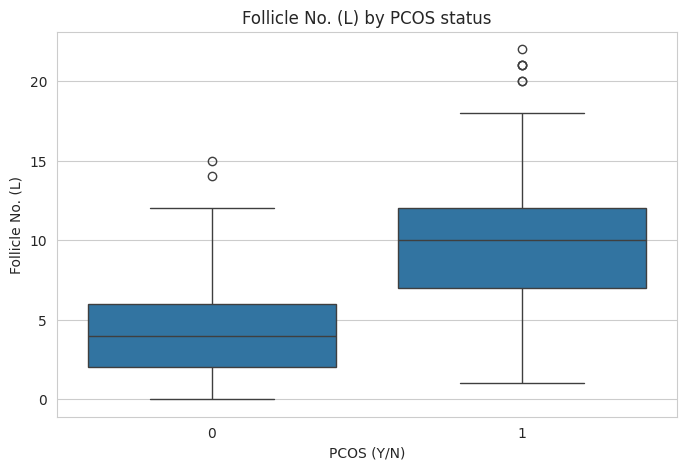
\includegraphics[width=0.85\linewidth]{figs/fig_follicle_r_boxplot.png}
\caption{Right-ovary follicle count by PCOS status.}
\label{fig:follicle_r}
\end{figure}

\begin{figure}[htbp]
\centering
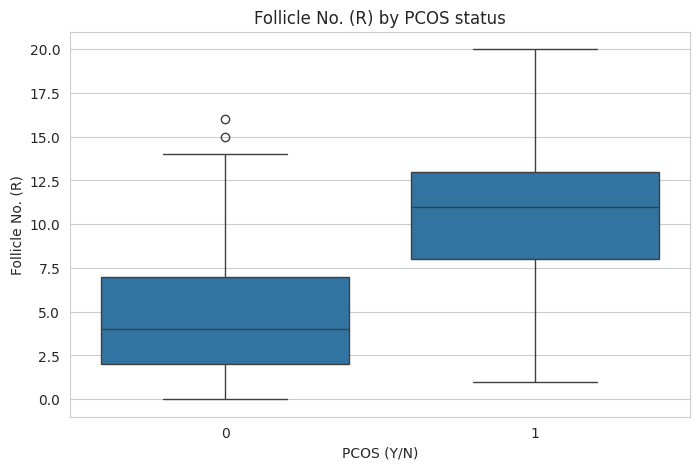
\includegraphics[width=0.85\linewidth]{figs/fig_follicle_l_boxplot.png}
\caption{Left-ovary follicle count by PCOS status.}
\label{fig:follicle_l}
\end{figure}

\begin{figure}[htbp]
\centering
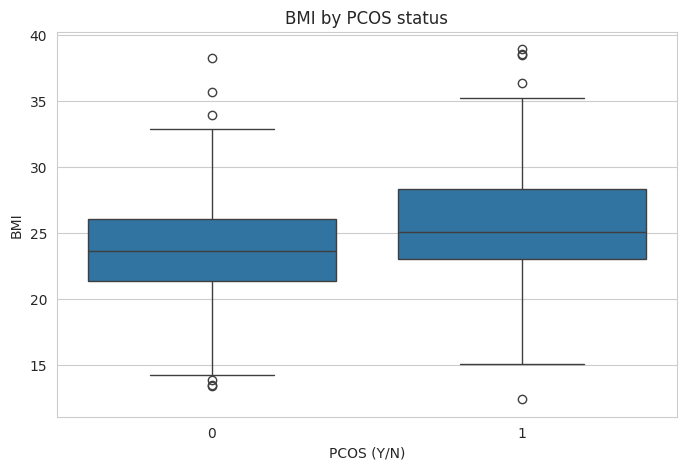
\includegraphics[width=0.85\linewidth]{figs/fig_bmi_boxplot.png}
\caption{BMI by PCOS status.}
\label{fig:bmi}
\end{figure}

\subsection{Model Comparison}

Table~\ref{tab:results} summarizes performance across all evaluated models. All three primary classifiers achieved ROC-AUC between 0.949 and 0.956. XGBoost achieved the highest point estimates on accuracy, precision, and F1-score; however, a paired $t$-test on cross-validated ROC-AUC scores between XGBoost and Random Forest showed no statistically significant difference ($p = 0.322$). Hyperparameter tuning (randomized search over 30 configurations), SMOTE-based class balancing, and soft-voting ensembling were additionally evaluated as robustness checks; none produced a statistically meaningful improvement over the default-configuration models, with several variants performing marginally worse (Table~\ref{tab:results}, rows 5--8), consistent with the models already approaching a performance ceiling given the modest dataset size ($n=541$).

\begin{table}[htbp]
\caption{Model Comparison Summary}
\label{tab:results}
\centering
\small
\begin{tabular}{@{}lccccc@{}}
\toprule
\textbf{Model} & \textbf{Acc.} & \textbf{Prec.} & \textbf{Rec.} & \textbf{F1} & \textbf{AUC} \\
\midrule
Logistic Regression        & 0.890 & 0.816 & 0.861 & 0.838 & 0.951 \\
Random Forest (all feat.)  & 0.917 & 0.966 & 0.778 & 0.862 & 0.949 \\
XGBoost (all feat.)        & 0.936 & 0.968 & 0.833 & 0.896 & 0.956 \\
RF (top 10 features)       & 0.917 & 0.909 & 0.833 & 0.870 & 0.943 \\
RF (tuned)                 & 0.899 & 0.963 & 0.722 & 0.825 & 0.942 \\
XGBoost (tuned)            & 0.899 & 0.903 & 0.778 & 0.836 & 0.955 \\
RF + SMOTE                 & 0.899 & 0.879 & 0.806 & 0.841 & 0.933 \\
Ensemble (RF + XGB, tuned) & 0.908 & 0.933 & 0.778 & 0.848 & 0.951 \\
RF (independent holdout)   & 0.902 & 0.828 & 0.889 & 0.857 & 0.984 \\
\bottomrule
\end{tabular}
\end{table}

An additional, independently-drawn holdout split (15\% of the data, unseen during any tuning or feature selection decision) yielded ROC-AUC $= 0.984$ (Table~\ref{tab:results}, final row). Given the modest size of this holdout partition ($n \approx 81$), this figure is best interpreted alongside the cross-validated estimate (mean ROC-AUC $= 0.961 \pm 0.010$) as evidence of performance stability across data splits, rather than as a higher ``true'' accuracy in isolation.

Figure~\ref{fig:cm} and Figure~\ref{fig:roc} show the confusion matrix and ROC curve for the Random Forest model on the primary test partition.

\begin{figure}[htbp]
\centering
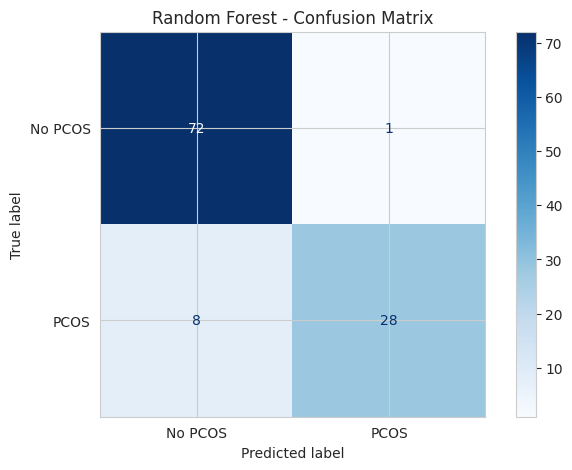
\includegraphics[width=0.85\linewidth]{figs/fig_confusion_matrix.png}
\caption{Confusion matrix, Random Forest (primary test set).}
\label{fig:cm}
\end{figure}

\begin{figure}[htbp]
\centering
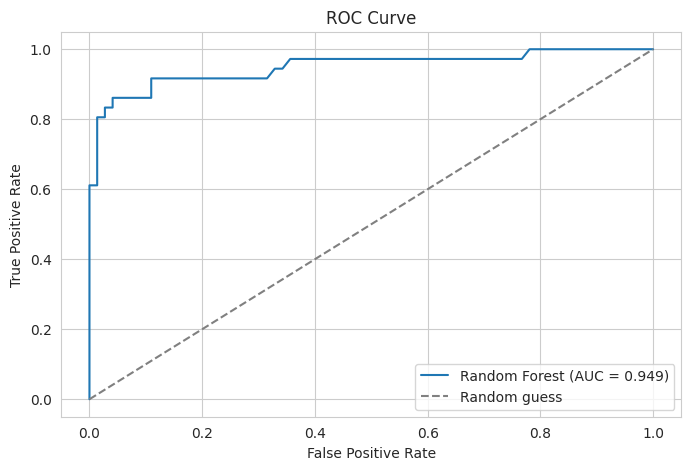
\includegraphics[width=0.85\linewidth]{figs/fig_roc_curve.png}
\caption{ROC curve, Random Forest (AUC $=0.949$).}
\label{fig:roc}
\end{figure}

\subsection{Feature Reduction and Cross-Model Agreement}

SHAP analysis of the Random Forest model (Fig.~\ref{fig:shap_bar}, Fig.~\ref{fig:shap_beeswarm}) identified right- and left-ovary follicle count as the two dominant predictors by a substantial margin, followed by weight gain, skin darkening, hair growth, cycle length, AMH, cycle regularity, fast food consumption, and acne (Table~\ref{tab:top10}).

\begin{figure}[htbp]
\centering
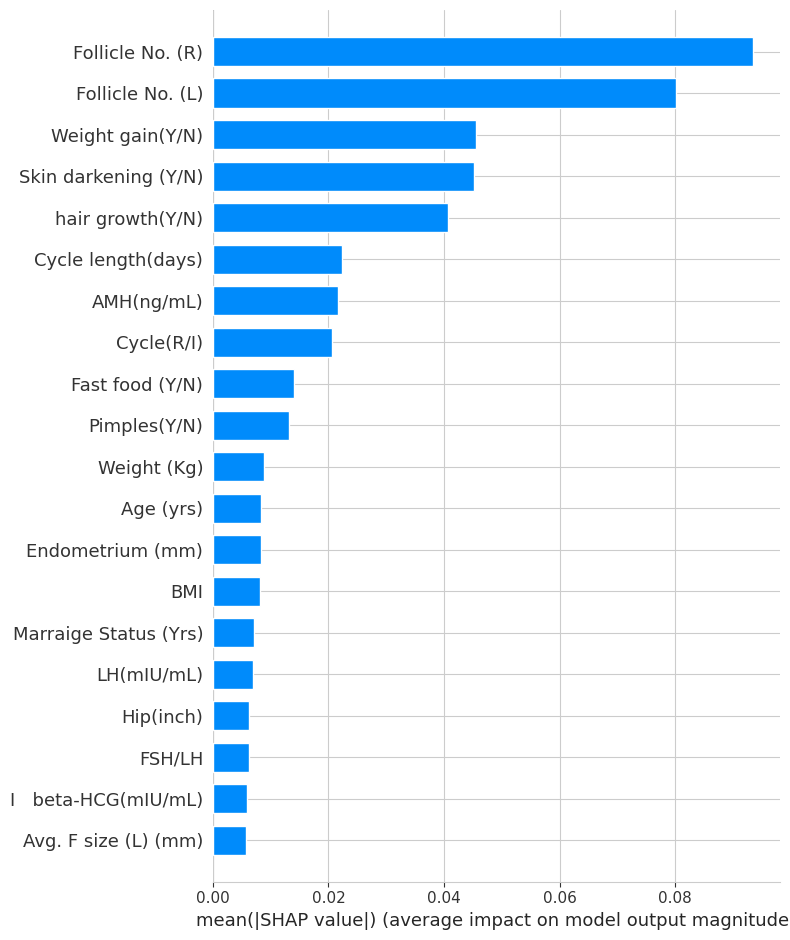
\includegraphics[width=0.95\linewidth]{figs/fig_shap_bar_rf_full.png}
\caption{Mean absolute SHAP value by feature, Random Forest (full feature set).}
\label{fig:shap_bar}
\end{figure}

\begin{figure}[htbp]
\centering
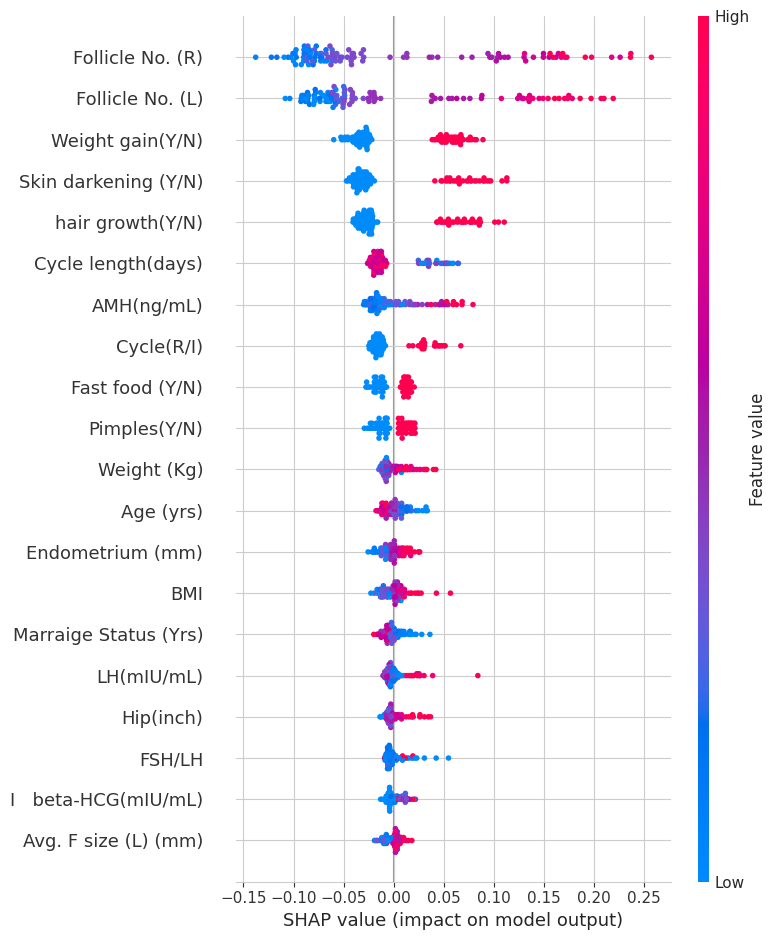
\includegraphics[width=0.95\linewidth]{figs/fig_shap_beeswarm.png}
\caption{SHAP summary (beeswarm) plot, Random Forest. Color indicates feature value; horizontal position indicates impact on model output.}
\label{fig:shap_beeswarm}
\end{figure}

\begin{table}[htbp]
\caption{Top 10 Features by Random Forest SHAP Importance}
\label{tab:top10}
\centering
\small
\begin{tabular}{@{}lc@{}}
\toprule
\textbf{Feature} & \textbf{Mean $|$SHAP$|$} \\
\midrule
Follicle No. (R)     & 0.0935 \\
Follicle No. (L)     & 0.0802 \\
Weight gain (Y/N)    & 0.0455 \\
Skin darkening (Y/N) & 0.0452 \\
Hair growth (Y/N)    & 0.0406 \\
Cycle length (days)  & 0.0224 \\
AMH (ng/mL)          & 0.0217 \\
Cycle (R/I)          & 0.0207 \\
Fast food (Y/N)      & 0.0140 \\
Pimples (Y/N)        & 0.0132 \\
\bottomrule
\end{tabular}
\end{table}

Retraining Random Forest on only these 10 features yielded ROC-AUC $= 0.943$, versus $0.949$ for the full 44-feature model -- a difference of 0.006. A paired $t$-test on cross-validation folds confirmed this difference was not statistically significant ($p = 0.893$), indicating that the 10-feature model is statistically indistinguishable in performance from the full-feature model, while requiring roughly one-quarter of the clinical measurements.

To assess whether this feature ranking was an artifact of the Random Forest algorithm specifically, SHAP importance was independently computed for XGBoost (Fig.~\ref{fig:shap_xgb}) and Logistic Regression (Fig.~\ref{fig:shap_lr}), and feature ranks were compared across all three models (Table~\ref{tab:crossmodel}).

\begin{figure}[htbp]
\centering
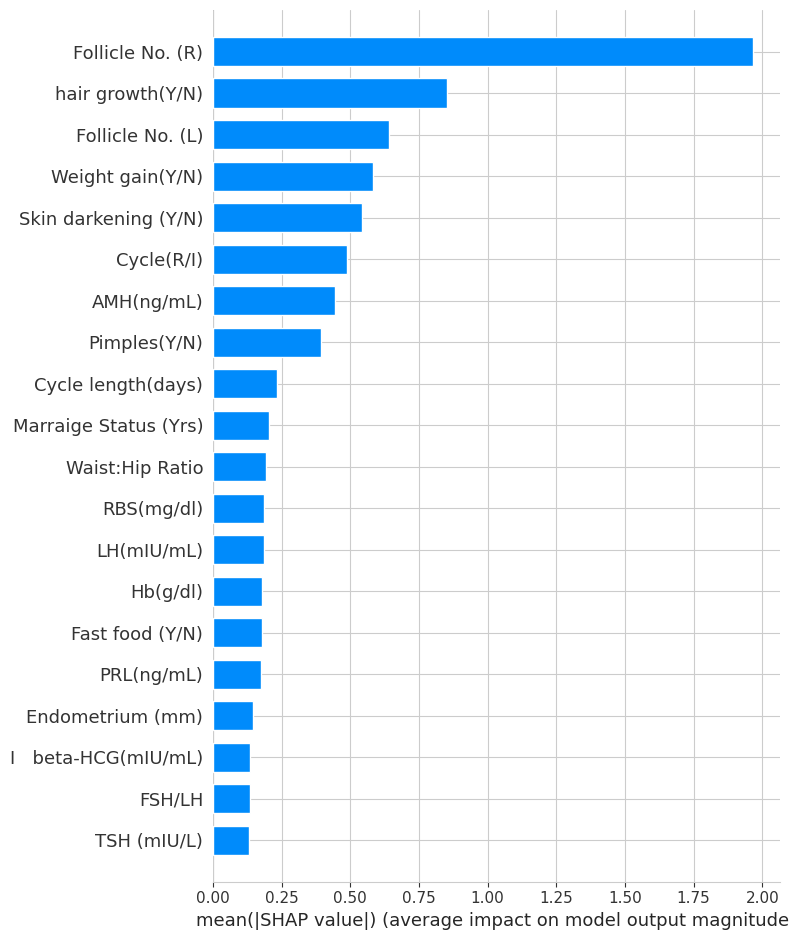
\includegraphics[width=0.95\linewidth]{figs/fig_shap_xgb.png}
\caption{Mean absolute SHAP value by feature, XGBoost.}
\label{fig:shap_xgb}
\end{figure}

\begin{figure}[htbp]
\centering
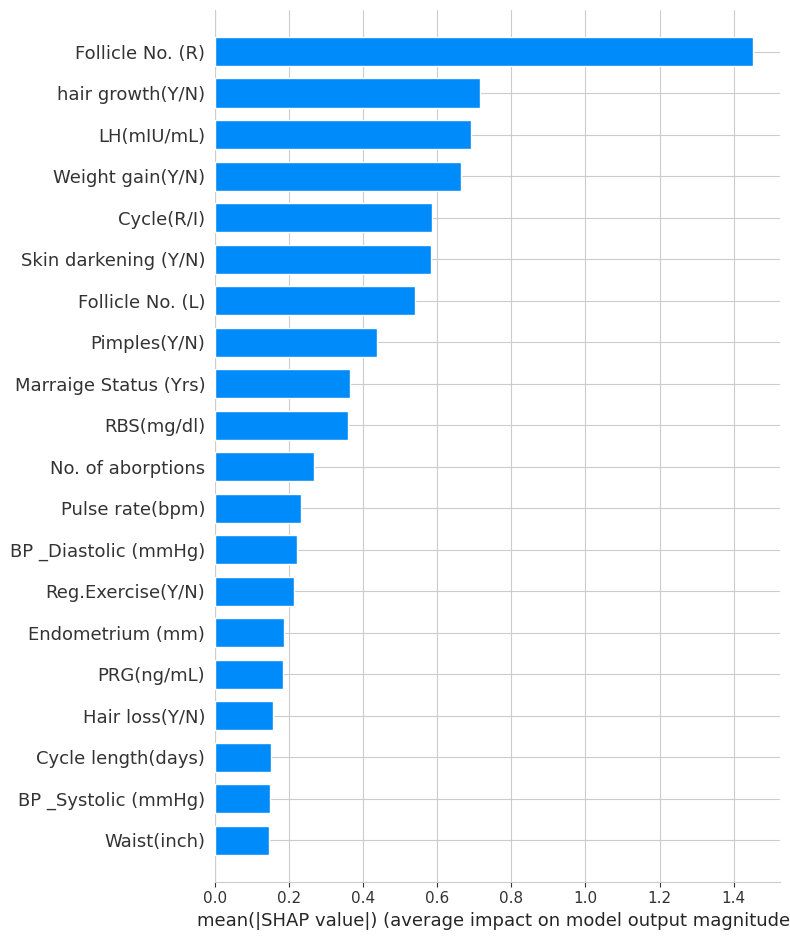
\includegraphics[width=0.95\linewidth]{figs/fig_shap_lr.png}
\caption{Mean absolute SHAP value by feature, Logistic Regression.}
\label{fig:shap_lr}
\end{figure}

\begin{table}[htbp]
\caption{Cross-Model Feature Rank Comparison (1 = most important)}
\label{tab:crossmodel}
\centering
\small
\begin{tabular}{@{}lccc@{}}
\toprule
\textbf{Feature} & \textbf{RF} & \textbf{XGBoost} & \textbf{LogReg} \\
\midrule
Follicle No. (R)     & 1  & 1  & 1  \\
Follicle No. (L)     & 2  & 3  & 7  \\
Weight gain (Y/N)    & 3  & 4  & 4  \\
Skin darkening (Y/N) & 4  & 5  & 6  \\
Hair growth (Y/N)    & 5  & 2  & 2  \\
Cycle length (days)  & 6  & 9  & 18 \\
AMH (ng/mL)          & 7  & 7  & 22 \\
Cycle (R/I)          & 8  & 6  & 5  \\
Fast food (Y/N)      & 9  & 15 & 24 \\
Pimples (Y/N)        & 10 & 8  & 8  \\
\bottomrule
\end{tabular}
\end{table}

Right-ovary follicle count was ranked the single most important feature by all three models regardless of architecture, and six of the ten features showed broad agreement across models. Notably, AMH and cycle length -- ranked highly by both tree-based models -- were ranked far lower by Logistic Regression (22nd and 18th, respectively), suggesting these features may relate to PCOS status non-linearly, a relationship that tree-based models can capture natively but a linear model cannot without explicit feature engineering.

\subsection{Threshold Optimization}

At the default 0.5 classification threshold, Random Forest achieved 77.8\% recall. Analysis of the precision--recall trade-off curve (Fig.~\ref{fig:pr}) identified an adjusted threshold of 0.345, at which recall improved to 91.7\% while precision remained at 80.5\% -- a substantially more clinically appropriate operating point for a screening application, where failing to flag a true case is generally costlier than a false alarm requiring follow-up testing.

\begin{figure}[htbp]
\centering
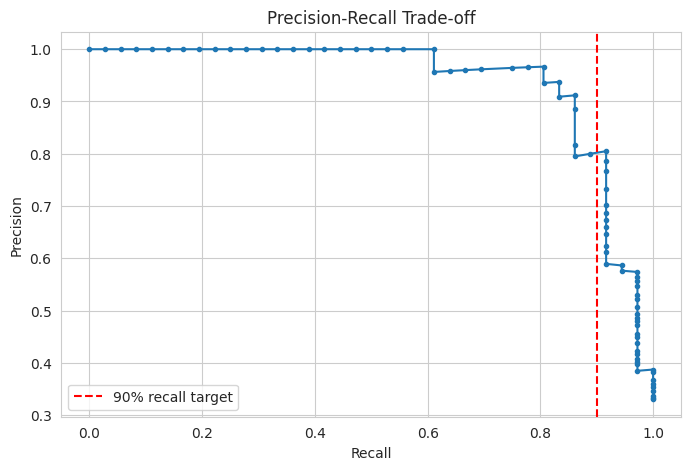
\includegraphics[width=0.85\linewidth]{figs/fig_pr_tradeoff.png}
\caption{Precision--recall trade-off curve, Random Forest.}
\label{fig:pr}
\end{figure}

\subsection{Calibration Analysis}

Figure~\ref{fig:calibration} shows calibration curves for all three models. Logistic Regression tracked closest to the ideal diagonal across the probability range, indicating its predicted probabilities most closely reflect true empirical likelihoods. Random Forest showed moderate deviation, while XGBoost -- despite achieving the highest raw discriminative performance -- showed the largest deviation from perfect calibration, consistently underestimating true PCOS likelihood in the low-to-moderate predicted-probability range.

\begin{figure}[htbp]
\centering
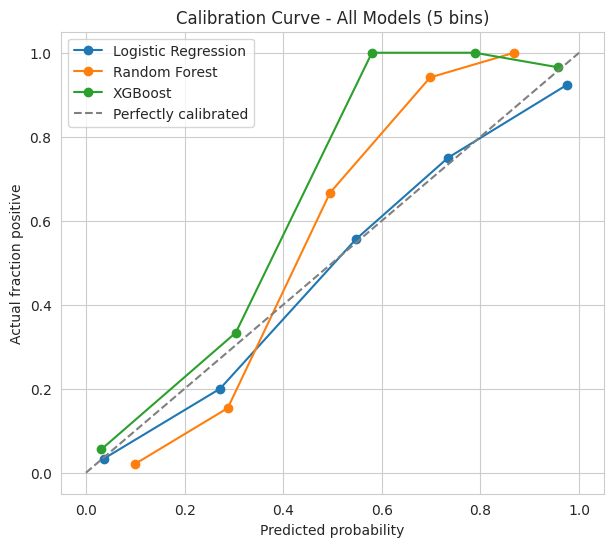
\includegraphics[width=0.85\linewidth]{figs/fig_calibration.png}
\caption{Calibration curves for Logistic Regression, Random Forest, and XGBoost (5 bins).}
\label{fig:calibration}
\end{figure}

This is a substantive finding: it indicates that the model with the best point-estimate accuracy is not necessarily the model best suited to applications where the numeric probability value itself is clinically consumed (e.g., communicating individualized risk to a patient), as opposed to applications requiring only a binary flag.

\subsection{Interactive Prototype}

To assess practical deployability of the reduced 10-feature model, a web-based interactive prototype was implemented using Streamlit and deployed publicly. Fig.~\ref{fig:app1} shows the input interface, and Fig.~\ref{fig:app2} shows a correctly classified high-risk example (follicle counts of 14 and 12, weight gain, irregular cycle, skin darkening, hair growth, and elevated AMH), returning a 93.5\% predicted probability of PCOS -- consistent with predictions obtained directly from the underlying trained model, confirming correct end-to-end deployment. A prominent disclaimer clarifies that the tool is a research prototype and not a validated diagnostic instrument.

\begin{figure}[htbp]
\centering
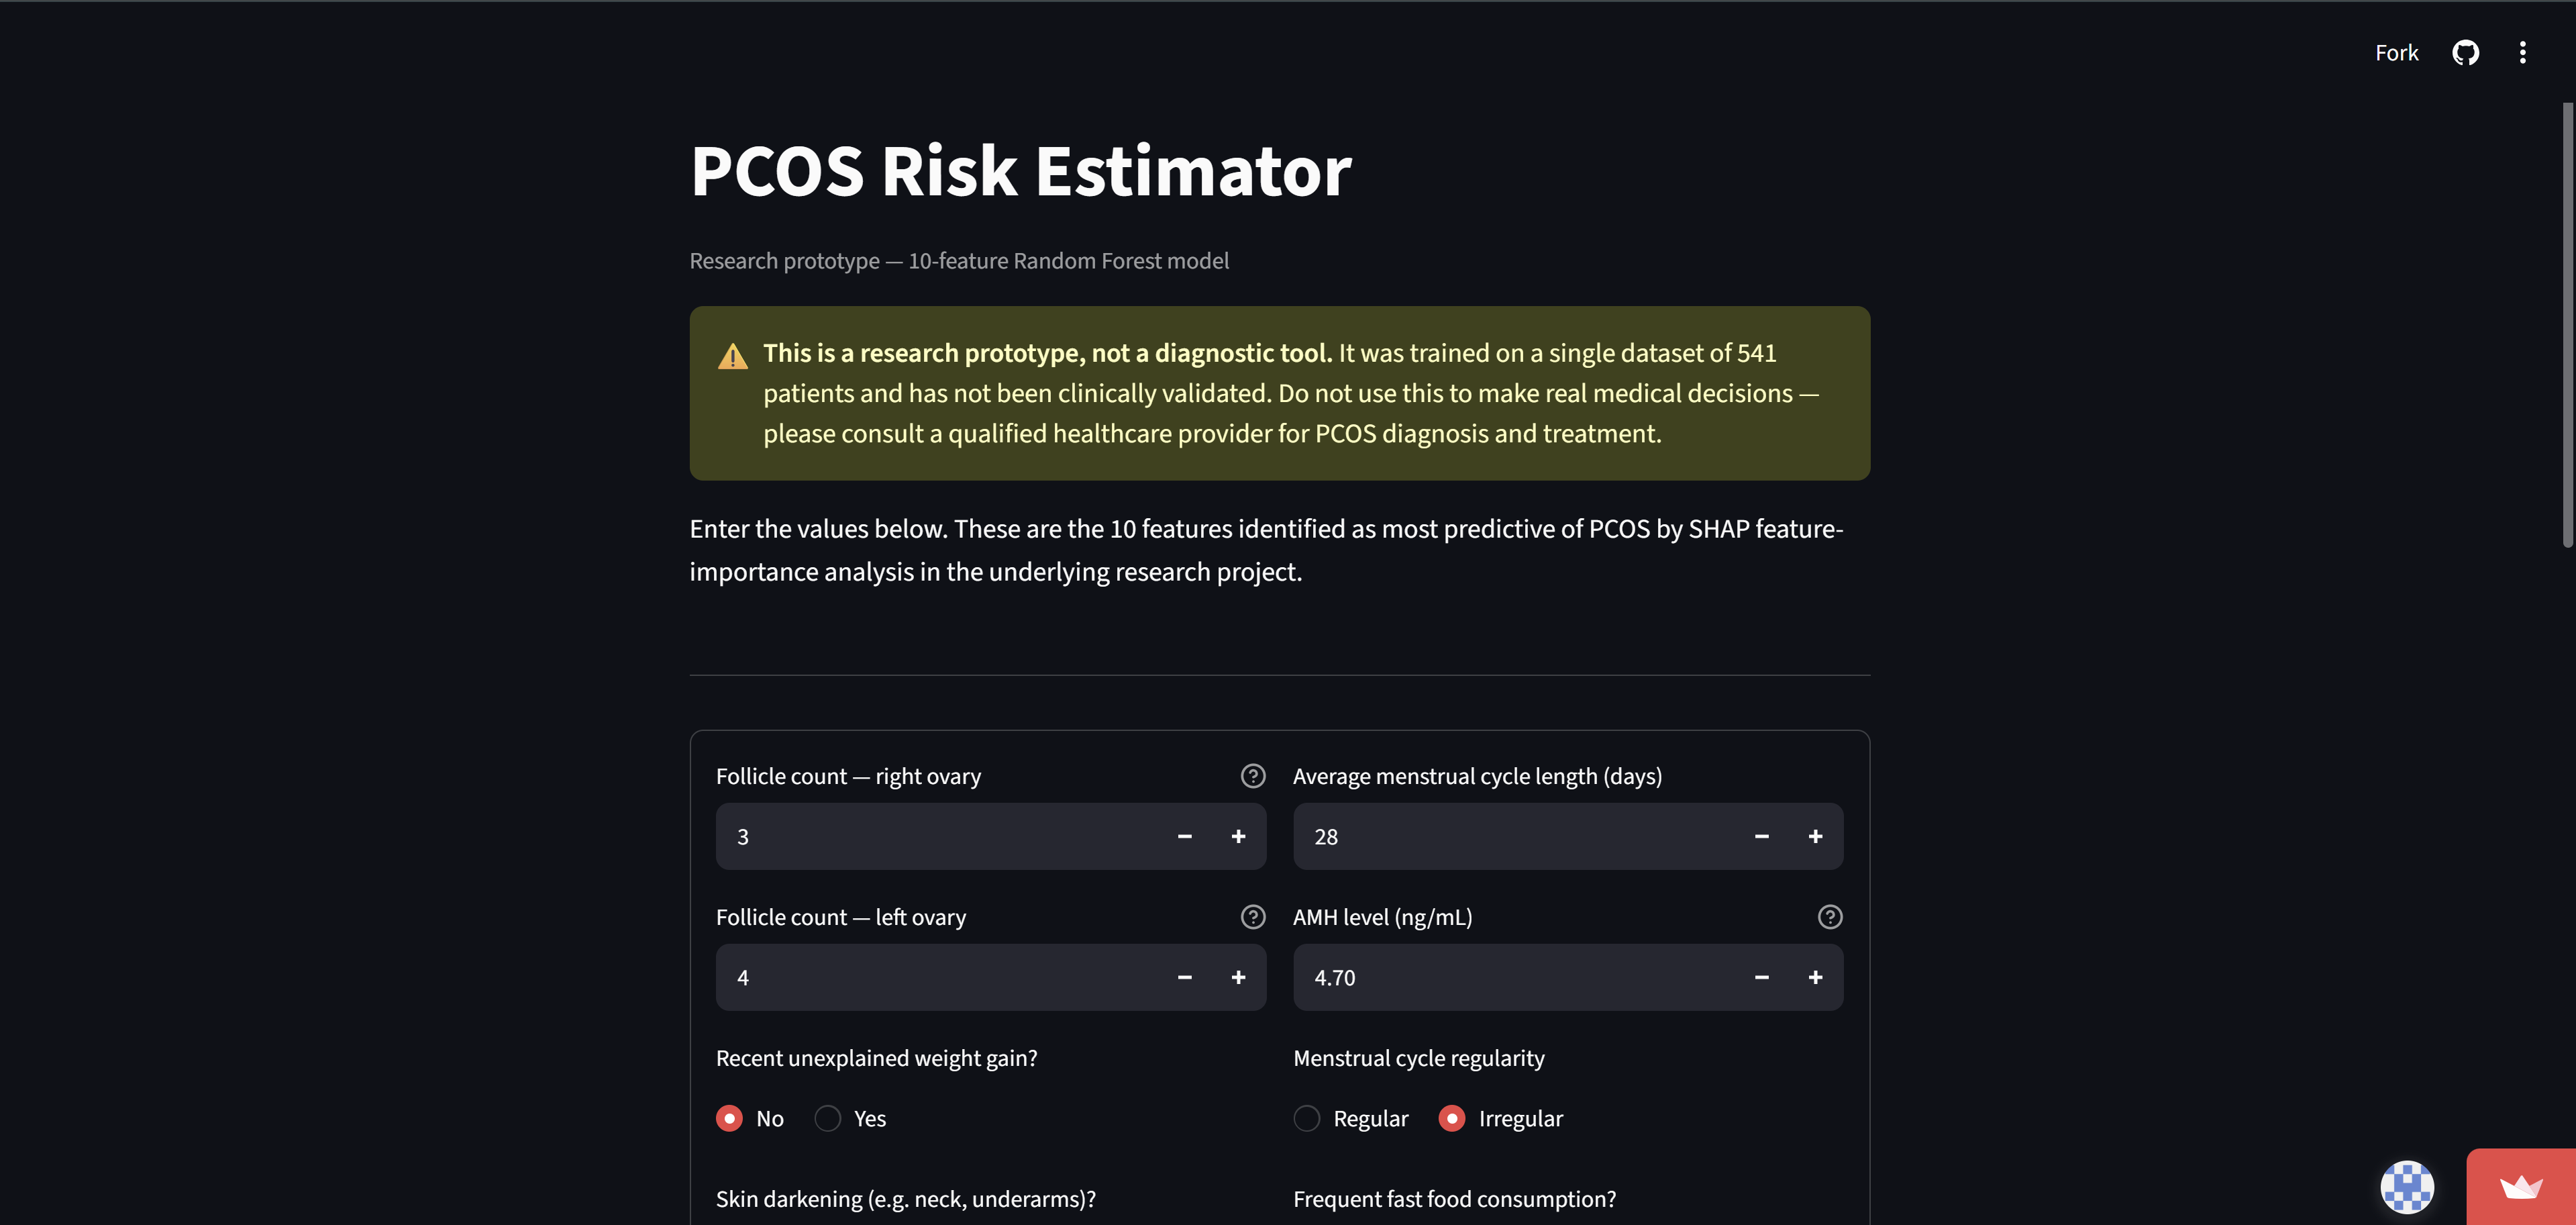
\includegraphics[width=\linewidth]{figs/fig_app_form1.png}
\caption{Interactive prototype input interface, showing the 10 reduced features and research-use disclaimer.}
\label{fig:app1}
\end{figure}

\begin{figure}[htbp]
\centering
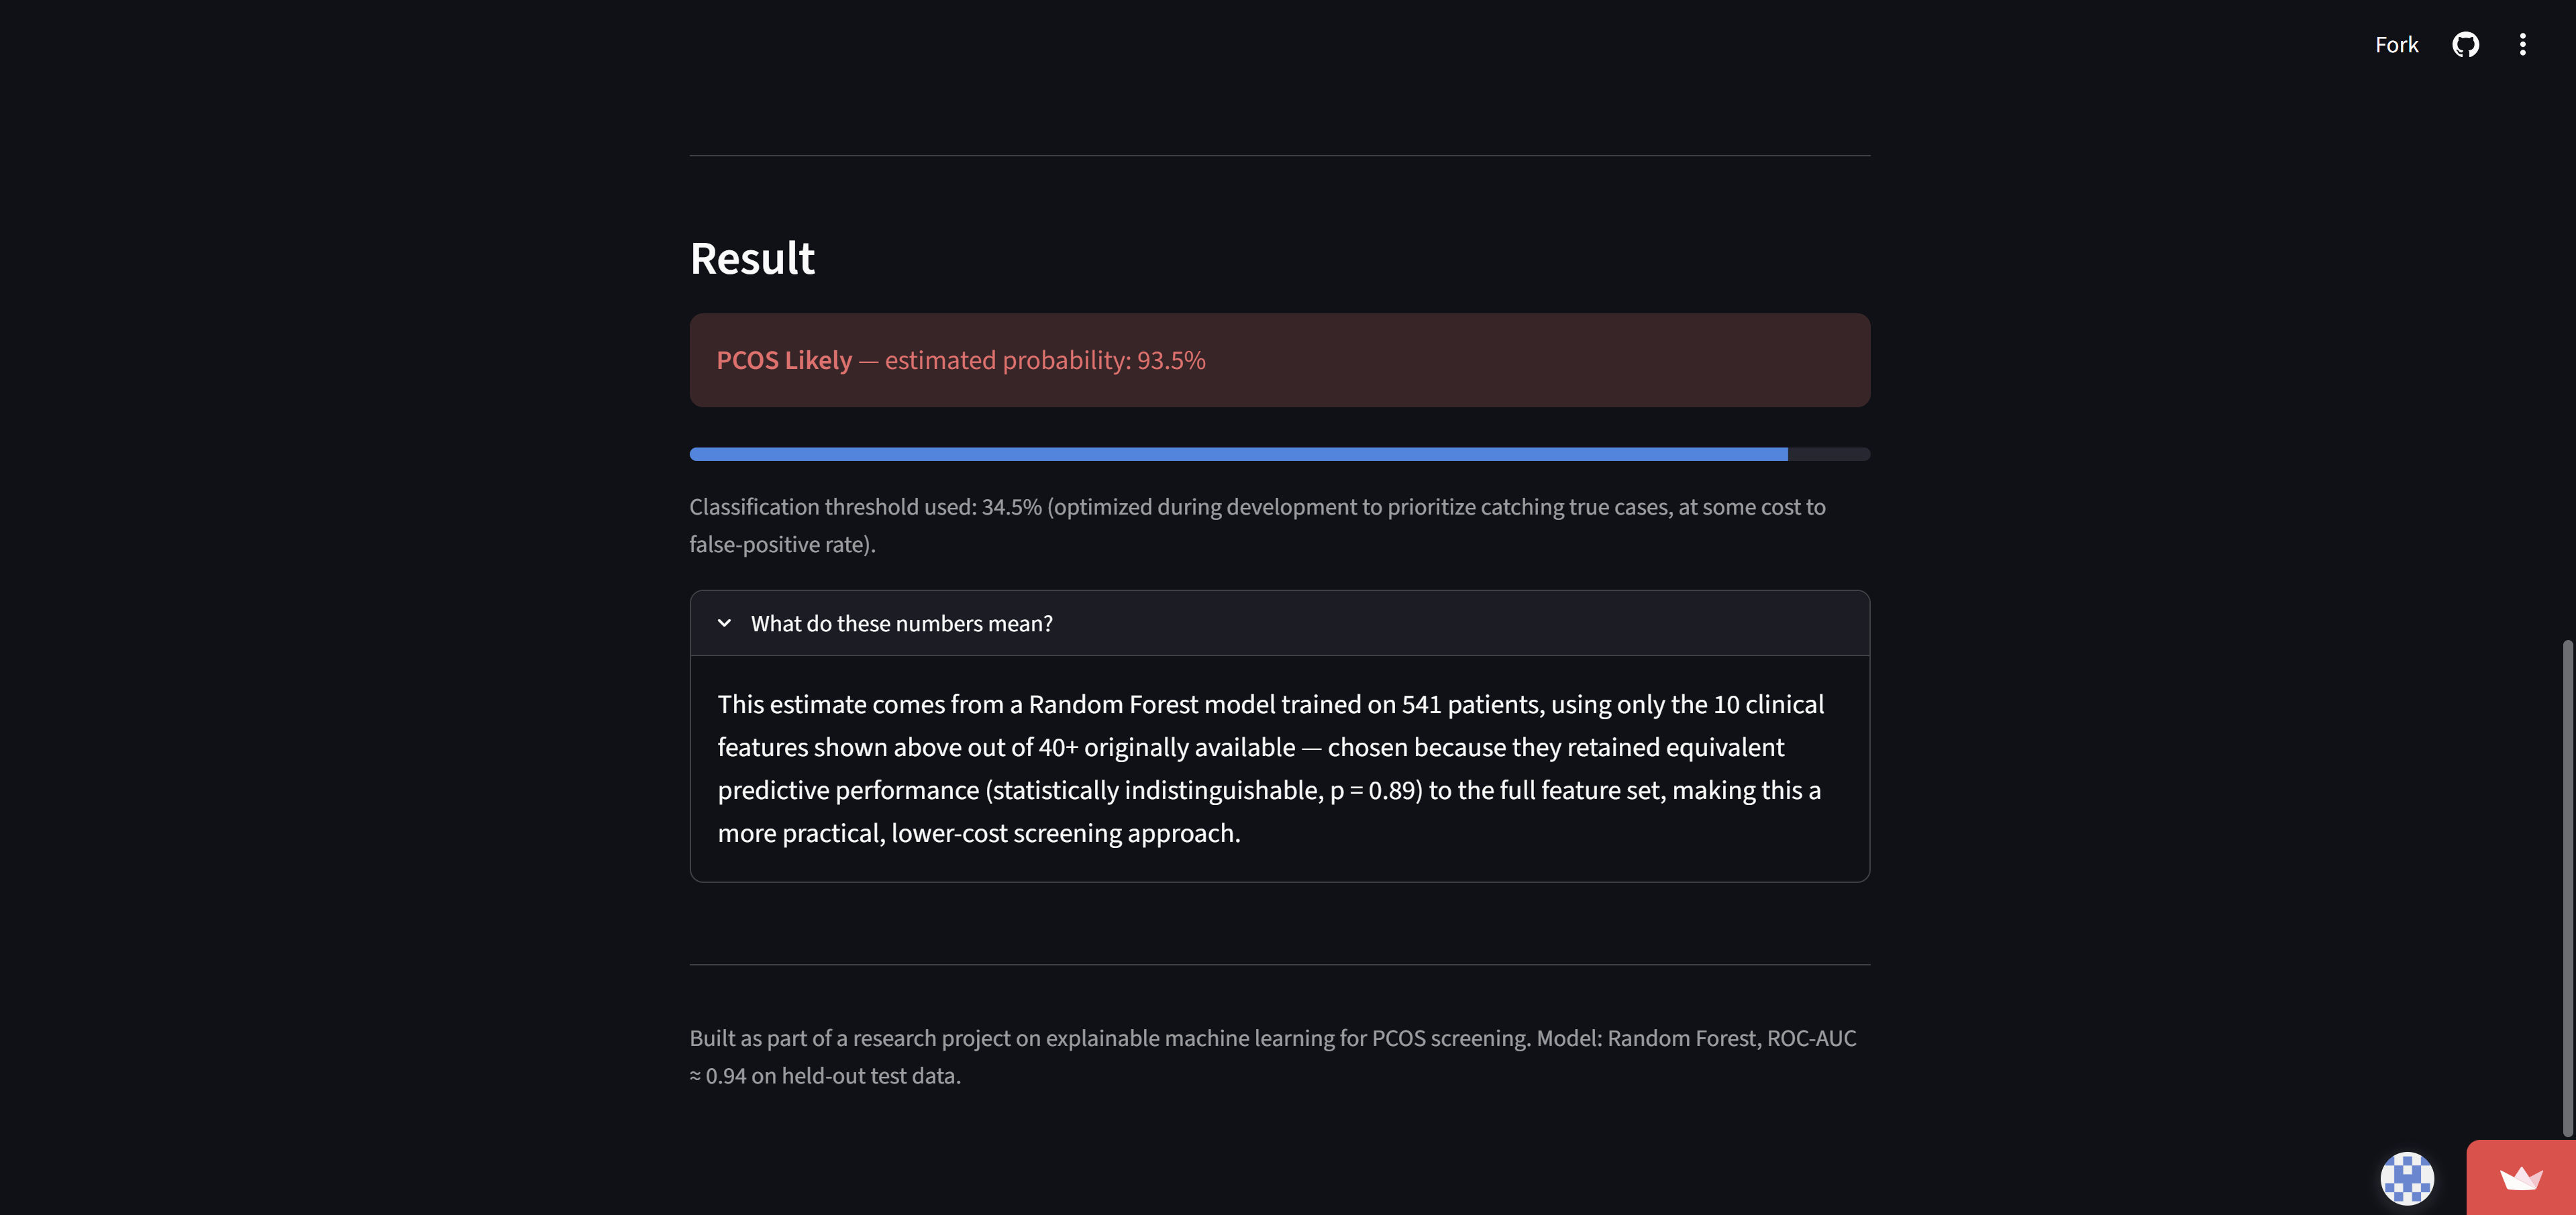
\includegraphics[width=\linewidth]{figs/fig_app_result_positive.png}
\caption{Prototype output for a high-risk clinical profile (predicted probability 93.5\%).}
\label{fig:app2}
\end{figure}

\section{Discussion}

The central finding of this study is that model architecture and feature count matter less than commonly assumed for this diagnostic task, provided the right features are retained. Three structurally different classifiers converged on statistically indistinguishable performance, and a 75\% reduction in feature count produced no statistically significant performance cost. This has direct practical relevance: a screening tool requiring only follicle counts, four binary symptom indicators, cycle length, AMH, cycle regularity, and dietary habit -- omitting numerous additional hormonal panel measurements present in the original dataset -- is meaningfully cheaper and faster to administer in resource-constrained clinical settings, without a demonstrated loss of diagnostic reliability.

The calibration finding adds an important qualification often absent from prior PCOS-ML literature: the model that appeared ``best'' by conventional accuracy-oriented metrics (XGBoost) was simultaneously the model whose probability outputs were least trustworthy at face value. This distinction matters because clinical deployment context determines which property is more important -- a binary triage flag can tolerate poor calibration if discrimination is strong, whereas a tool intended to communicate individualized numeric risk to a patient cannot.

Several robustness checks -- hyperparameter tuning, SMOTE-based rebalancing, and ensembling -- were evaluated and found not to improve, and in some cases marginally worsened, performance relative to default-configuration models. We report this as a substantive negative result rather than omitting it: it suggests the dataset size, not model configuration, is the binding constraint on further improvement, directing future effort toward data acquisition rather than continued algorithmic tuning.

\subsection{Limitations}

This study has several limitations that should inform interpretation of its findings. First, all primary results derive from a single-source dataset ($n=541$) collected across hospitals in one geographic region; external validation on an independent, geographically distinct patient cohort was not feasible within the scope of this work, a limitation also explicitly noted as an open gap in recent PCOS-AI systematic reviews \cite{ghaderzadeh2025}. An independent dataset ($n=684$) was examined for this purpose but was found to use categorical, self-reported hormonal assessments (including an ``unknown'' response option) rather than quantitative laboratory measurements, and critically lacked follicle count entirely -- the single strongest predictor identified in this study -- rendering direct cross-dataset validation infeasible without substantial feature-schema harmonization. This itself illustrates a broader, field-level barrier to external validation in PCOS-ML research: heterogeneity in feature availability and measurement quality across publicly available datasets.

Second, calibration analysis was conducted on a modest test partition ($n \approx 108$), and calibration curves computed with finer binning were visibly unstable, improving only when bin count was reduced -- indicating that reliable calibration assessment for this task requires substantially larger sample sizes than are currently available. Third, attempts to correct model calibration using isotonic regression did not yield a consistent improvement, plausibly for the same sample-size reasons. Fourth, the class distribution in the primary dataset (67\% PCOS-positive) may not reflect general-population prevalence (reported at 8--13\% \cite{ghaderzadeh2025}), and prevalence mismatch between training data and deployment population can affect real-world predictive value even when discrimination metrics remain strong.

\section{Conclusion}

This study demonstrates that explainable machine learning can meaningfully simplify PCOS screening without sacrificing statistical performance, and that model interpretability, feature efficiency, and probability calibration -- not solely raw accuracy -- should be treated as first-class evaluation criteria in clinical ML research. A 10-feature Random Forest model, validated as statistically equivalent to a 44-feature model and cross-checked for feature-importance consistency across three model architectures, was translated into a deployed interactive prototype demonstrating practical feasibility. Future work should prioritize multi-site data collection with harmonized feature schemas to enable genuine external validation, larger-scale calibration assessment, and prospective clinical evaluation before any such tool could be considered for real-world screening use.

\section*{Availability}

The interactive prototype described in Section IV-F is publicly accessible at:
\begin{center}
\footnotesize\url{https://pcos-prediction-app-9d2phrtrhqdagalxyu7yts.streamlit.app/}
\end{center}
Source code and the trained model are available upon request. This tool is a research prototype only and is not validated for clinical diagnostic use.

\begin{thebibliography}{00}

\bibitem{ghaderzadeh2025} M. Ghaderzadeh \emph{et al.}, ``Artificial intelligence in polycystic ovary syndrome: a systematic review of diagnostic and predictive applications,'' \emph{BMC Medical Informatics and Decision Making}, vol. 25, no. 427, 2025. doi: 10.1186/s12911-025-03255-6.

\bibitem{rotterdam2004} Rotterdam ESHRE/ASRM-Sponsored PCOS Consensus Workshop Group, ``Revised 2003 consensus on diagnostic criteria and long-term health risks related to polycystic ovary syndrome (PCOS),'' \emph{Fertility and Sterility}, vol. 81, no. 1, pp. 19--25, 2004.

\bibitem{barrera2023} F. J. Barrera, E. D. L. Brown, A. Rojo, J. Obeso, H. Plata, E. P. Lincango, N. Terry, R. Rodr\'{i}guez-Guti\'{e}rrez, J. E. Hall, and S. Shekhar, ``Application of machine learning and artificial intelligence in the diagnosis and classification of polycystic ovarian syndrome: a systematic review,'' \emph{Frontiers in Endocrinology}, vol. 14, 2023. doi: 10.3389/fendo.2023.1106625.

\bibitem{mohiuddin2025} M. Uddin, ``Early PCOS detection: A comparative analysis of traditional and ensemble machine learning models with advanced feature selection,'' \emph{Engineering Reports}, Wiley, 2025. doi: 10.1002/eng2.70008.

\bibitem{webbased2024} ``Empowering early detection: A web-based machine learning approach for PCOS prediction,'' \emph{Intelligent Systems with Applications / ScienceDirect}, 2024.

\bibitem{breiman2001} L. Breiman, ``Random forests,'' \emph{Machine Learning}, vol. 45, no. 1, pp. 5--32, 2001.

\bibitem{chen2016} T. Chen and C. Guestrin, ``XGBoost: A scalable tree boosting system,'' in \emph{Proc. 22nd ACM SIGKDD Int. Conf. Knowledge Discovery and Data Mining}, 2016, pp. 785--794.

\bibitem{lundberg2017} S. M. Lundberg and S.-I. Lee, ``A unified approach to interpreting model predictions,'' in \emph{Advances in Neural Information Processing Systems}, vol. 30, 2017.

\bibitem{kottarathil} P. Kottarathil, ``Polycystic ovary syndrome (PCOS),'' Kaggle dataset, 2020. [Online]. Available: https://www.kaggle.com/datasets/prasoonkottarathil/polycystic-ovary-syndrome-pcos

\end{thebibliography}

\end{document}
